\documentclass[a4paper,11pt]{article}

\usepackage{a4wide}

\usepackage{amsmath,bm}
\newcommand{\td}{\mathrm{d}}
\newcommand{\te}{\mathrm{e}}
\newcommand{\ti}{\mathrm{i}}
\newcommand{\sinc}{\mathrm{sinc}}
\usepackage{tikz}

\begin{document}

\setcounter{tocdepth}{5}
\tableofcontents

\section{Laplace kernel}

\subsection{2D case}

\begin{equation}
G({\bf y}, {\bf x}) = -\frac{\ln |{\bf y}-{\bf x}|}{2\pi} = -\frac{\ln r}{2\pi}
\end{equation}

\subsubsection{Collocation}

\paragraph{Constant line SLP}

\begin{equation}
\lim_{\epsilon \to 0} \left( \int_{-d_1}^{-\epsilon} G(r) \td r + \int_{\epsilon}^{d_2} G(r) \td r \right)
=
\frac{d_1(1-\ln d_1) + d_2(1-\ln d_2)}{2\pi}
\end{equation}

\paragraph{Constant line HSP}

\begin{align}
\frac{\partial}{\partial n_x}
\int_{-d_1}^{d_2} 
\frac{\partial}{\partial n_y}
\frac{-\ln |r|}{2\pi}
\td y 
&=
\frac{\partial}{\partial z}
\int_{-d_1}^{d_2} 
\frac{-1}{2\pi r} \frac{(y, -z) \cdot (0,1)}{r}
\td y \nonumber \\
&=
\frac{1}{2\pi} \frac{\partial}{\partial z}
\int_{-d_1}^{d_2} 
\frac{z}{\left(y^2+z^2\right)}
\td y \nonumber \\
&=
\frac{1}{2\pi} \frac{\partial}{\partial z}
\left[
\tan^{-1}\left(d_2/z\right)
-
\tan^{-1}\left(-d_1/z\right)
\right]
\nonumber \\
&=
\frac{1}{2\pi} \frac{\partial}{\partial z}
\left[
\tan^{-1}\left(d_2/z\right) + \tan^{-1}\left(d_1/z\right)
\right]
\nonumber \\
&=
\frac{1}{2\pi} 
\left[
\frac{-d_2}{d_2^2+z^2} + \frac{-d_1}{d_1^2+z^2}
\right]
\nonumber \\
& \to
\frac{-1}{2\pi} 
\left[
\frac{1}{d_2} + \frac{1}{d_1}
\right]
\end{align}


\subsubsection{Galerkin}

\paragraph{Face match}

\subparagraph{Constant line SLP}

\begin{equation}
\int_{0}^{d}
\lim_{\epsilon \to 0}
\left(
\int_{0}^{x-\epsilon} G(x-y) \td y
+
\int_{x+\epsilon}^{d} G(x-y) \td y
\right)
\td x
=
d^2\frac{3-2\ln d}{4\pi}
\end{equation}

\subparagraph{Linear line SLP}

\begin{equation}
\int_{0}^{d} N_i(x) \int_{0}^{d} G(x-y) N_j(y) \td y \td x
=
\frac{d^2}{32\pi} \begin{bmatrix}
7-4 \ln d & 5 - 4 \ln d \\
5-4 \ln d & 7 - 4 \ln d
\end{bmatrix}
\end{equation}

\paragraph{Edge match}

\subparagraph{Constant line SLP kernel}

\begin{multline}
\int_{S_{x}} \int_{S_{y}} G(r) \td S_y \td S_x =
\int_{0}^{d_1} \int_{0}^{d_2}
\ln \sqrt{(x+y \cos\phi)^2 + (y\sin\phi)^2}
\td y \td x \\
=
\frac{
c \left(d_1^2 \ln \frac{d_1}{d_3} + {d_2}^2 \ln \frac{d_2}{d_3}\right)
+ s \left(d_1^2 q(d_1, d_2, \phi) + d_2^2 q(d_2, d_1, \phi)\right)
+ d_1 d_2 \left(3 - 2 \ln d_3 \right)
}{
4 \pi
}
\end{multline}
%
where
%
\begin{equation}
q(d_1, d_2, \phi) = \tan^{-1}\left(\frac{d_2 + d_1 \cos\phi}{d_1 \sin\phi}\right) - \tan^{-1}\left(\cot\phi\right)
\end{equation}

\subparagraph{Constant line DLP kernel}

\begin{multline}
\int_{S_{x}} \int_{S_{y}} G'(r) r'_{n_{y}} \td S_y \td S_x =
\int_{0}^{d_1} \int_{0}^{d_2}
\frac{x\sin\phi}{(x+y \cos\phi)^2 + (y\sin\phi)^2}
\td y \td x \\
=
\frac{1}{2\pi}\left(-d_1 q(d_1, d_2, \phi) + d_2 \cos\phi q(d_2, d_1, \phi)
- d_2 \sin\phi \ln \frac{d_3}{d_2}\right)
\end{multline}

\subsection{3D case}

\begin{equation}
G(r) = \frac{1}{4\pi r}
\end{equation}

\subsubsection{Collocation over constant triangle}

\begin{equation}
\int_0^{2\pi} \int_0^{R(\theta)} \frac{r \td r \td \theta}{4\pi r}
=
\frac{1}{4\pi}\int_0^{2\pi} R(\theta) \td \theta
\end{equation}
%
The angular integral is split up into three integrals, each over one triangular domain.
One triangle is displayed below, $\bf x_0$ denotes the collocational point:

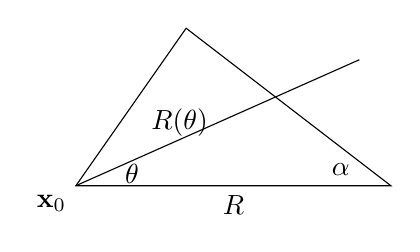
\begin{tikzpicture}[scale=2]
\path [draw] (0,0) node [anchor = north east] {${\bf x}_0$} -- node [anchor = north] {$R$} (2,0) -- (.7, 1) -- cycle;
\path [draw] (0,0) -- node [anchor = east] {$R(\theta)$} (1.8,.8);
\path (.25,-.05) node [anchor = south west] {$\theta$};
\path (1.8,0) node [anchor = south east] {$\alpha$};
\end{tikzpicture}

From the law of sines, $R(\theta)$ is expressed as
%
\begin{equation}
R(\theta) = \frac{R \sin(\alpha)}{\sin(\theta+\alpha)}
\end{equation}
%
using the identity
%
\begin{equation}
\int \frac{\td x}{\sin x} = \log \tan (x/2)
\end{equation}
%
the integral can be expressed (by summing for the three triangles) as follows:
%
\begin{equation}
I = \frac{1}{4\pi} \sum_{i = 1}^3
R_i \sin\alpha_i \left[ \log \left( \frac{\tan\left(\frac{\phi_i+\alpha_i}{2}\right)}{\tan\left(\frac{\alpha_i}{2}\right)}\right)\right]
\end{equation}


\begin{align}
\frac{\partial}{\partial n_x}
\int
\frac{\partial}{\partial n_y}
G(r)
\td y
&=
\frac{\partial}{\partial z}
\int
\frac{-1}{4\pi \left(r^2_{2D} + z^2\right)}
\frac{({\bf r}_{2D},-z)\cdot({\bf 0},1)}{\sqrt{r^2_{2D} + z^2}}
\td {\bf y}
\nonumber \\
&=
\frac{1}{4\pi}
\frac{\partial}{\partial z}
\int
\frac{z}{\left(r^2_{2D} + z^2\right)^{3/2}}
\td {\bf y}
\nonumber \\
&=
\frac{1}{4\pi}
\frac{\partial}{\partial z}
\int_{0}^{2\pi}
\int_{0}^{R(\theta)}
\frac{r_{2D} z}{\left(r^2_{2D} + z^2\right)^{3/2}}
\td r_{2D}
\td \theta
\nonumber \\
&=
\frac{-1}{4\pi}
\frac{\partial}{\partial z}
\int_{0}^{2\pi}
\left(
\frac{z}{\sqrt{R(\theta)^2 + z^2}}
-
1
\right)
\td \theta
\nonumber \\
&=
\frac{-1}{4\pi}
\int_{0}^{2\pi}
\frac{\partial}{\partial z}
\frac{z}{\sqrt{R(\theta)^2 + z^2}}
\td \theta
\nonumber \\
&=
\frac{-1}{4\pi}
\int_{0}^{2\pi}
\left(
\frac{\sqrt{R(\theta)^2 + z^2} - \frac{z}{2\sqrt{R(\theta)^2 + z^2}}}{R(\theta)^2 + z^2}
\right)
\td \theta
\nonumber \\
&\to
\frac{-1}{4\pi}
\int_{0}^{2\pi}
\frac{1}{R(\theta)}
\td \theta
\end{align}


\section{Analytical singular integrals of the Helmholtz kernel}

\subsection{2D case}

The Helmholtz kernel in 2D reads as
%
\begin{equation}
G(r) = -\frac{\ti}{4}H^{(2)}_0(k|r|)
\end{equation}
%
where $H_0^{(2)}$ denotes the Hankel function of the second kind, defined using the Bessel functions of the first and second kinds:
%
\begin{equation}
H^{(2)}_0(z) = J_0(z) - \ti Y_0(z)
\end{equation}


\subsubsection{Collocation over constant line}

In order to integrate the 2D Green's function over a constant line with the singularity in the line's center, the series expansions of the Bessel functions are needed:
%
\begin{align}
J_0(z) &= \sum_{n=0}^{\infty} (-1)^n \frac{q^{2n}}{\left(n!\right)^2} \\
Y_0(z) &= \frac{2}{\pi} \left[
	\left(\ln q +\gamma\right)J_0(z)
	-
	\sum_{n=1}^{\infty} (-1)^{n} b_n \frac{q^{2n}}{\left(n!\right)^2}
\right]
\end{align}
%
where
%
\begin{equation}
q = z/2, \qquad b_n = \sum_{k=1}^n \frac{1}{k}, \qquad \gamma = \lim_{n\to\infty} b_n - \ln n
\end{equation}

Substituting the series expansions into the definition of the Hankel function results in:
%
\begin{equation}
H^{(2)}_0(z) =
\left[1 - \frac{2 \ti}{\pi} \left(\ln q +\gamma\right) \right]	
+
\sum_{n=1}^{\infty} (-1)^n \frac{q^{2n}}{\left(n!\right)^2}
\left[1 - \frac{2 \ti}{\pi} \left(\ln q +\gamma - b_n\right) \right]
\end{equation}
%
multiplying by $-\ti/4$ yields the series expansion of the Green's function
%
\begin{multline}
G(r) = \frac{-1}{2\pi} \left\{
\left[\ti\pi/2 + \ln q +\gamma \right]	
+ \left(\sum_{n=1}^{\infty}
(-1)^n \frac{q^{2n}}{\left(n!\right)^2}
\left[\ti\pi/2 + \gamma - b_n \right]	\right) \right. \\
\left.
+
\left(\sum_{n=1}^{\infty}
(-1)^n \frac{q^{2n}\left(\ln q\right)}{\left(n!\right)^2}
\right)
\right\}
\end{multline}

Obviously, the singularity is because of the term $\ln q$. In order to cancel the singularity, the static part of the Green's function is subtracted, resulting in the regular term
%
\begin{multline}
G(r)-G_0(r) = \frac{-1}{2\pi} \left\{
\left[\ti\pi/2 + \ln \left(k/2\right) +\gamma \right]	
+ 
\left(\sum_{n=1}^{\infty}
(-1)^n \frac{q^{2n}}{\left(n!\right)^2}
\left[\ti\pi/2 + \gamma - b_n \right]	\right) \right. \\
\left.
+
\left(\sum_{n=1}^{\infty}
(-1)^n \frac{q^{2n} \ln q}{\left(n!\right)^2}
\right)
\right\}
\end{multline}
%
This regular power series can be integrated analytically:
%
\begin{multline}
2\int_{0}^{R} G(r)-G_0(r) \td r
= \\
\frac{-R}{\pi} \left\{
\left[\ti\pi/2 + \ln \left(k/2\right) +\gamma \right]
+
\sum_{n=1}^{\infty}
\frac{(-1)^n Q^{2n}}{\left(n!\right)^2\left(2n+1\right)}
\left[\ti\pi/2 + \gamma - b_n + \ln Q - \frac{1}{2n + 1}\right]
\right\}
\end{multline}
%
where $Q = kR/2$.

Finally, adding the integral of the static part to the regular integral, the power series simplifies to
%
\begin{multline}
2\int_{0}^{R} G(r)-G_0(r) \td r + \frac{R}{\pi}\left(1-\ln R\right)
= \\
\frac{-R}{\pi} 
\sum_{n=0}^{\infty}
\frac{(-1)^n Q^{2n}}{\left(n!\right)^2\left(2n+1\right)}
\left[\ti\pi/2 + \gamma + \ln Q - b_n - \frac{1}{2n + 1}\right]
\end{multline}
%
where the definition of $b_n$ has been modified by including the $b_0 = 0$ term.


\subsection{3D case}

\begin{equation}
G(r) = \frac{\te^{-\ti k r}}{4\pi r}
\end{equation}

\subsubsection{Collocation over constant triangle}

The singular integral over a triangle is regularised by subtracting and adding the static ($k = 0$) part
%
\begin{equation}
G(r) = \frac{1}{4\pi r} -\ti k \te^{-\ti k r/2} \frac{\sinc(k r/2)}{4\pi}
\end{equation}
%
The static part is integrated analytically.
The dynamic part is regular and can be integrated using a low order Gaussian quadrature over the triangle.


\begin{equation}
G''_{n_x, n_y} = \frac{G}{r^2} \left[ 
\left(1+\ti k r\right)\left(n_x n_y + r'_{n_x} r'_{n_y}\right) 
 + \left(2 + 2 \ti k r - (kr)^2\right) r'_{n_x} r'_{n_y}
\right]
\end{equation}
%
and on a plane triangle
%
\begin{equation}
G''_{n_x, n_y} = \frac{G}{r^2} \left(1+\ti k r\right)
\end{equation}
%
We again subtract the static part, as well as the static Green's function $G_0(r)$ multiplied by $k^2/2$ to obtain a regular function represented by its Taylor series:
%
\begin{equation}
G''_{n_x, n_y} - {G_0}''_{n_x, n_y} - \frac{k^2}{2} G_0 =
-\frac{\ti k^3}{4\pi}
\left(
\frac{1}{3}
- \frac\gamma{8} 
+ \frac{\gamma^2}{30} 
- \frac{\gamma^3}{144} 
+ \frac{\gamma^4}{840} 
-\frac{\gamma^5}{5760} 
+\dots
\right)
\end{equation}
%
where $\gamma = \ti k r$


\section{General singular}

General shape set, general element shape ($L$-set)
%
\begin{equation}
\int_S G({\bf x}-{\bf x}_0) N({\bf x}) \td S
\end{equation}
%
Reference system
%
\begin{equation}
\int_{\Sigma} G({\bf x}(\bm{\xi})-{\bf x}_0) N(\bm{\xi}) J(\bm{\xi}) \td \Sigma
\end{equation}
%
Polar transform
%
\begin{equation}
\int_{0}^{2\pi}
\int_{\alpha(\varepsilon,\theta)}^{R(\theta)}
G({\bf x}(\bm{\xi}(\rho,\theta))-{\bf x}_0) N(\bm{\xi}(\rho,\theta)) J(\bm{\xi}(\rho,\theta)) \rho
\td \rho
\td \theta
=
\int_{0}^{2\pi}
\int_{\alpha(\varepsilon,\theta)}^{R(\theta)}
F(\rho, \theta)
\td \rho
\td \theta
\end{equation}

$F$ expressed using its Laurent series:
%
\begin{equation}
F(\rho, \theta)
= \frac{F_{-2}(\theta)}{\rho^2}
+ \frac{F_{-1}(\theta)}{\rho}
+ O(1)
\end{equation}
%
\begin{multline}
I =
\int_{0}^{2\pi}
\int_{0}^{R(\theta)}
\underbrace{
F(\rho, \theta) - \frac{F_{-2}(\theta)}{\rho^2} - \frac{F_{-1}(\theta)}{\rho}
}_{O(1)}
\td \rho
\td \theta \\
+
\int_{0}^{2\pi}
F_{-2}(\theta)
\left(
\frac{1}{\alpha(\varepsilon,\theta)}
-\frac{1}{R(\theta)}
\right)
\td \theta
+
\int_{0}^{2\pi}
F_{-1}(\theta)
\ln \left|\frac{R(\theta)}{\alpha(\varepsilon,\theta)}\right|
\td \theta
\end{multline}
%
\begin{multline}
I =
\int_{0}^{2\pi}
\int_{0}^{R(\theta)}
F(\rho, \theta) - \frac{F_{-2}(\theta)}{\rho^2} - \frac{F_{-1}(\theta)}{\rho}
\td \rho
\td \theta
-
\int_{0}^{2\pi}
\frac{F_{-2}(\theta)}{R(\theta)}
\td \theta \\
+
\int_{0}^{2\pi}
F_{-2}(\theta)
\frac{1}{\varepsilon\beta(\theta) + \varepsilon^2\gamma(\theta)}
\td \theta
+
\int_{0}^{2\pi}
F_{-1}(\theta)
\ln \left|\frac{R(\theta)}{\beta(\theta)}\right|
\td \theta
-
\ln \varepsilon
\underbrace{
\int_{0}^{2\pi}
F_{-1}(\theta)
\td \theta}_0
\end{multline}

%
\begin{multline}
I =
\int_{0}^{2\pi}
\int_{0}^{R(\theta)}
F(\rho, \theta) - \frac{F_{-2}(\theta)}{\rho^2} - \frac{F_{-1}(\theta)}{\rho}
\td \rho
\td \theta  \\
-
\int_{0}^{2\pi}
F_{-2}(\theta)\left(\frac{1}{R(\theta)}
+
\frac{\gamma(\theta)}{\beta^2(\theta)}
\right)
\td \theta
+
\int_{0}^{2\pi}
F_{-1}(\theta)
\ln \left|\frac{R(\theta)}{\beta(\theta)}\right|
\td \theta
\end{multline}

\begin{align}
\beta(\theta) &= \frac{1}{A(\theta)} \\
\gamma(\theta) &= -\frac{{\bf A}(\theta) \cdot {\bf B}(\theta)}{A^4(\theta)}
\end{align}


\subsection{Specialisation to 3D potential kernels}

Assumptions: The element is smooth and the singular point is internal.
%
\begin{equation}
F = \frac{-{\bf r} \cdot {\bf J} N \rho}{4\pi r^3}
\end{equation}
%
\begin{equation}
F_{-2}(\theta) = F_{-1}(\theta) = 0
\end{equation}
%
meaning that simple Duffy quadrature is accurate.

\begin{equation}
F = \frac{
\left[
\left({\bf J} \cdot {\bf n}_{x_0}\right)
-
3 \left(\nabla r \cdot {\bf J}\right) \left(-\nabla r \cdot {\bf n}_{x0}\right)
\right] N \rho
}{
4\pi r^3
}
\end{equation}
%
\begin{align}
F_{-2}(\theta) &= \frac{J_0 N_0}{4\pi A^3(\theta)} \\
F_{-1}(\theta) &= \left(\frac{{\bf J}_0 N_1(\theta) + {\bf J}_1(\theta) N_0}{4\pi A^3(\theta)}
-\frac{3 N_0 {\bf J}_0 \left({\bf A}(\theta) \cdot {\bf B}(\theta)\right)}{4\pi A^5(\theta)}\right) {\bf n}_{x_0}
\end{align}

\end{document}

